% !TeX root = ./main.tex
% ~ 3 pages

\section{System Model}
\label{sec:system_model}

In this section, we develop an analytical model to derive the three metrics that constitute the objective functions of our VNFPP given in~\pref{sec:problem_formulation}. They can be calculated for each service by examining the queues in the network. Each data center component consists of one or more buffers where packets are queued before being served. The arrival and service rates at a data center component determine the expected length of each queue, which in turn determine the waiting time and the probability of packet loss as well as the energy consumption. This information can then be used to calculate the latency, packet loss and energy consumption for each path of each service. In the following paragraphs, we first derive the approximation of the arrival rate for each data center component, based on which we calculate the three metrics. %considered in our VNFPP.

%\begin{algorithm}[t]
%	\KwData{Services $S$, service paths $R^s$, path selection probabilities $\mathbb{P}_{R^s}$, packet drop probabilities $\mathbb{P}^d_c$, service arrival rate $\lambda_s$}
%
%	\For{$s \in\mathcal{S}$} {
%		\For{$i \gets 0$ \KwTo $|\mathcal{R}^s|$} {
%
%			$\lambda \gets \lambda_{s} \cdot \mathbb{P}_{R^s_i}$ \tcp{Set route arrival rate}
%
%			\For{$c \in R^s_i$} {
%				$\lambda_{c} \gets \lambda_{c} + \lambda$ \tcp{Add rate to component}
%
%				$\lambda \gets \lambda \cdot (1 - \mathbb{P}_c^d)$ \tcp{Set departing rate}
%			}
%		}
%	}
%
%	\caption{Calculate the instantaneous expected arrival rates of all components}
%	\label{alg:calc_inst_arr}
%\end{algorithm}

\subsection{Arrival Rates of Data Center Components}
\label{sec:arrival_rate}

To calculate the arrival rate we must establish some reasonable assumptions about the system's behavior. In line with \cite{PoissonTraffic}, we assume the traffic generated by end users follows a Poisson distribution with a mean rate $\lambda_s$. As end users access the service independently, the total traffic arrival rate of a service can be calculated as the superposition of multiple independent Poisson processes. When packets arrive at a data center component, they are served with a first-in-first-out queueing strategy. To make the analytical model applicable to the practical implementation, instead of exploiting the infinite queueing strategies in \cite{InfiniteQueue}, we assume each data center component has a finite buffer length $B_c$. If the buffer becomes full, the newly arrived packets would be dropped to avoid system congestion. Finally, since packets are processed independently the time for a data center component to process a packet follows an exponential distribution with service rate $\mu_c$. Under these conditions, we model the service processing at each data center component as an M/M/1/B$_c$ system.

Next we can calculate the arrival rate of each data center component. Let $\lambda_c$ be the arrival rate of a data center component $c\in\mathcal{C}$. It is the sum of the packet flow rates of all paths entering this data center component. Due to the finite buffer size, the effective arrival rate $\lambda_c^e$ is less than the arrival rate and calculated as $\lambda _{ c }^{ e }=\lambda _{ c }{ \left( 1-\mathbb{P}^d_{c} \right)  }$, where $\mathbb{P}^d_{c}$ is the packet loss probability and is calculated as~\cite{Kleinrock75}:
\begin{equation}
    \mathbb{P}^d_{c}
	=
	\begin{cases}
		\frac{(1-\rho)\rho^{B_c}}{1-\rho^{B_c+1}}, & \text{if}\ \lambda\neq\mu\\
        \frac{1}{B_{c}+1}, & \text{otherwise}
	\end{cases},
	\label{eq:pl}
\end{equation}
where $\rho=\lambda_{c}/\mu_{c}$.

If the packet loss at a data center component were fixed then the arrival rate at each component would simply be the sum of the packet flow rates of the routes through that component. In practice, since the packet loss at a data center component depends on the arrival rate at the earlier components on the same path, dependency loops can form if the same component is visited multiple times in a sequence (as demonstrated in~\pref{fig:arrival_loop}). In this case, the packet loss probability at the revisited component becomes a function of its own arrival rate thus resulting in a dynamic system. Since the arrival rate at each component changes over time in a dynamic system, it is significantly more complex to derive the performance metrics based on the arrival rate. Existing works unfortunately neglect this factor by either considering models without packet loss (e.g., \cite{ZhangXLLGW17,QuZYSLR20,AgarwalMCD18}) or simply ignoring the dynamic feature of the system and only calculating the arrival rate at the outset instead (e.g.,~\cite{ChuaWZSH16,MarottaZDK17}). In this paper, we propose an iterative method to calculate the expected arrival rate over time. We first show that the arrival rates at all data center components naturally converge towards a fixed point given infinite time. Then, we elaborate the method that derives the expected arrival rate.

\begin{figure}[t!]
	\centering
	\begin{minipage}{0.24\textwidth}
		\centering
		\resizebox{0.9\textwidth}{!}{
			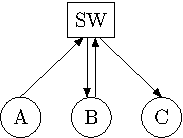
\includegraphics{figures/original_loop-crop}
		}
		\vspace{.2em}
		\subcaption{Original Configuration}
	\end{minipage}\hfill
	\vspace{2em}
	\begin{minipage}{0.24\textwidth}
		\centering
		\resizebox{0.9\textwidth}{!}{
			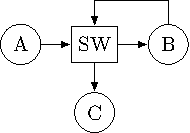
\includegraphics{figures/unfolded_loop-crop}
		}
		\vspace{.2em}
		\subcaption{Unfolded Loop}
	\end{minipage}

	\caption{Three VNFs (A, B, C) are visited in sequence through a single switch (SW). This forms a loop causing the arrival rate at the switch to be dependent on its own packet loss.}
	\label{fig:arrival_loop}
\end{figure}

\begin{lemma}
The arrival rate at each data center component converges towards a fixed point as time approach infinity.\footnote{The proof can be found in the Appendix B.}
\label{lemma:arrival_rate}
\end{lemma}

\begin{figure*}[t!]
	\centering
	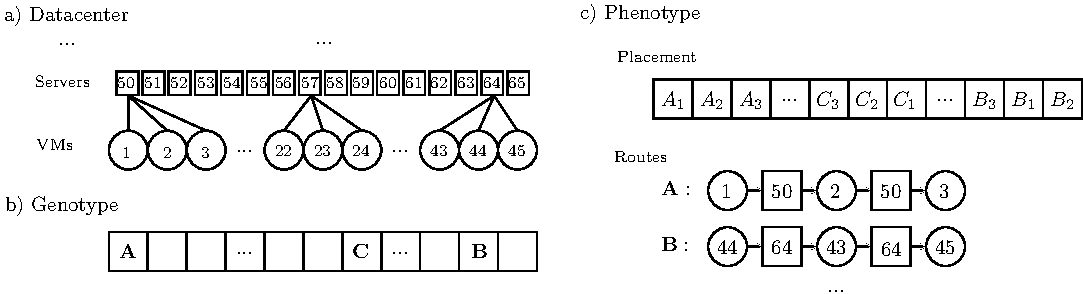
\includegraphics[width=\linewidth]{figures/solution_representation-crop}
	\caption{The genotype-phenotype solution representation used in this work.}
	\label{fig:gp_mapping}
\end{figure*}

%\begin{proof}
%Our proof considers a sequence of moments where the arrival rate is stable. We show that the instantaneous arrival rate $\lambda_t$ at any component at the time step $t$ is bounded by the arrival rates at the time steps $t-1$ and $t-2$. When $t\to\infty$, this bound converges towards a fixed value: %This is expressed as,
%\begin{equation}
%	\lim_{t\to\infty }{{\left|\lambda_{t-1}-\lambda_{t-2}\right|}}=0.
%\end{equation}
%%\noindent We show this by induction.
%
%Before carrying on our proof, we introduce the following two properties of the packet loss probability.
%\begin{itemize}
%	\item The packet loss probability strictly increases with the growth of arrival rate.
%	\item The packet loss probability asymptotically approaches $1$ with the growth of arrival rate.
%\end{itemize}
%
%Our proof is done by induction. We first prove that $\lambda_{t=2}$ is always bounded by $\lambda_{0}$ and $\lambda_{1}$ and then the inductive cases with $t\to \infty$. 
%
%When $t=0$, there is no packet in the queue, thus no packet is dropped. In this case, the effective arrival rate reaches its maximum. Furthermore, since the arrival rate is less than $\infty$ and the packet loss asymptotically approaches $1$, all future instances will have some packet lost where $\lambda_{t=0}>\lambda_{t>0}$. Since the effective arrival rate reaches its highest value at $t=0$, the packet loss probability at the next time step $\mathbb{P}^d_{t=1}$ must be the highest value. Hence, the effective arrival rate $\lambda_{t=1} < \lambda_{t>1}$. All in all, we have:
%\begin{equation}
%	\lambda_{t=1}<\lambda_{t=2}<\lambda_{t=0},
%\end{equation}
%where we denote $\lambda_{t=0}$ and $\lambda_{t=1}$ as the upper and lower bounds respectively.
%
%The inductive case consists of two parts.
%
%\begin{itemize}
%	\item We first show that if $\lambda_{t=n}$ is the lower bound of $\lambda$, then $\lambda_{t=n+1}$ will be the new upper bound. From the first property $\mathbb{P}^d_{t=n+1}<\mathbb{P}^d_{t=n}$, we have $\lambda_{t=n+1} > \lambda_{t=n}$. Furthermore, since $\lambda_{t=n} < \lambda_{t>n}$ and $\mathbb{P}^d_{t=n+1} < \mathbb{P}^d_{t>n+1}$, we have $\lambda_{t=n+1} > \lambda_{t>n}$ that makes $\lambda_{t=n+1}$ the new upper bound.
%	\item Secondly, we show that if $\lambda_{t=n}$ is the upper bound of $\lambda$, then $\lambda_{t=n+1}$ will be the new lower bound. From the first property $\mathbb{P}^d_{t=n+1} > \mathbb{P}^d_{t=n}$, we have $\lambda_{t=n+1}<\lambda_{t=n}$. Furthermore, since $\lambda_{t=n} > \lambda_{t>n}$ and $\mathbb{P}^d_{t=n+1}>\mathbb{P}^d_{t>n+1}$, we have $\lambda_{t=n+1}<\lambda_{t>n}$ that makes $\lambda_{t=n+1}$ the new lower bound.
%\end{itemize}
%
%Since the new upper and lower bounds of $\lambda$ are within the previous upper and lower bounds, they move towards each other at every time step and finally converge when $t\to \infty $.
%\end{proof}

A naive method of calculating the arrival rate, based on~\pref{lemma:arrival_rate}, is to evaluate the upper and lower bounds of the arrival rate until they converge. This is impractical since the theoretical result requires infinite time. Instead, this paper proposes to approximate the arrival rate by calculating the bounds until they converge to the point that further iterations are unlikely to change the expected arrival rate more than a threshold $\delta>0$. As the pseudo-code shown in Algorithm 2 in the Appendix C, it first initializes the packet loss at each data center component to 0 to simulate there being no packets in any queue (lines 3 to 4). In the main loop, the algorithm first calculates the current arrival rate and packet loss for each data center component by using the previous settings of packet loss (lines 6 to 8). From~\pref{lemma:arrival_rate}, we can see that the current arrival rate will be either a lower or upper bound of the arrival rate. Next the algorithm calculates the mean of the upper and lower bounds of the arrival rate for each data center component (line 12) and the divergence from the previous mean for each component (line 14). If the maximum divergence from the mean across all components has remained below $\delta$ for $\gamma>1$ iterations, future iterations are unlikely to alter the mean arrival rate. Hence, we terminate the process and output the mean arrival rate as the arrival rate at each data center component (lines 17 to 24).

Note that the parameters $\delta$ and $\gamma$ determine the accuracy and convergence speed of this model. A lower $\delta$ increases the model accuracy by requiring the mean to be more stable before being considered converged. The model is less sensitive to $\gamma$ which is required for the rare scenario where the bounds temporarily appear converged. We found that $\delta = 5.0$ and $\gamma = 10$ give a balanced trade-off between efficiency and accuracy. 

%\begin{algorithm}[t]
%	\KwData{Thresholds $\delta$ and $\gamma$}
%	\KwResult{Sets the arrival rate $\lambda_c$ for all components}
%	$N^i \gets 0$ \tcp{Sequential iterations below $\delta$}
%	
%	\For{$c \in C$}{
%		$\mathbb{P}^d_c \gets 0$ \tcp{Component packet loss}
%
%		$\overline{\lambda_c} \gets 0$ \tcp{Expected arrival rate}
%	}
%
%	Calculate $\lambda_c$ all components using \pref{alg:calc_inst_arr}
%	
%	\While{$N_{ci} < \gamma$}{
%
%		\For{$c \in C$}{
%			$\lambda^p_c \gets \lambda_c$  \tcp{Previous arrival rate of $c$}
%
%			Update $\mathbb{P}^d_c$ using $\lambda_c$ and \pref{eq:pl}
%		}
%
%		Update $\lambda_c$ of all components using \pref{alg:calc_inst_arr}
%
%		$M\!D \gets 0$ \tcp{Max. divergence}
%
%		\For{$c \in C$}{
%			\tcp{Calculate mean of current bounds}
%			$\overline{\lambda^p_c} \gets \left(\lambda^p_c + \lambda_c\right) /\ 2$
%
%			\tcp{Measure divergence of mean}
%			$D \gets \abs{\overline{\lambda^p_c} - \overline{\lambda_c}}$
%
%			\tcp{Update expected arrival rate}
%			$\overline{\lambda_c} \gets \overline{\lambda^p_c}$
%
%			\tcp{Update maximum divergence}
%			$M\!D \gets \textsc{Max}(D, M\!D)$
%		}
%
%		\eIf{$M\!D < \delta$}{
%			$N_{ci} \gets N + 1$
%		}{
%			$N_{ci} \gets 0$
%		}
%	}
%	
%	\tcp{Set final values of $\lambda_c$}
%	\For{$c \in C$}{
%		$\lambda_c \gets \overline{\lambda_c}$
%	}
%
%    % \Return $\lambda_c$
%	\caption{Calculate the stable expected arrival rates of all components}
%	\label{alg:calc_arr}
%\end{algorithm}

% However, if some loss of accuracy is permitted, we can closely approximate the fixed point by calculating the mean of the arrival rate over time until the change in the mean between time steps has remained less than a small amount $\delta$ for $\gamma$ iterations.

% \begin{lemma}
% The arrival rate calculation finishes in finite time if $\delta>0$ and $\gamma<\infty$.
% \end{lemma}

% \begin{proof}
% We prove this by showing any sequence of bound movements results in convergence. The bounds can either: 1) change by a small amount such that the mean does not change more than $\delta$, or 2) change by a large amount such that the \textit{does} change by more than $\delta$. In the first instance where there are $\gamma$ sequential small moves, the algorithm will terminate as the mean has changed by less than $\delta$ for $\gamma$ time steps. In the second instance, there are a finite number of large moves that can be performed before the bounds are too close for a large move to be possible and hence only small moves could occur. Likewise, any sequence of large and small moves must end with a sequence of small moves once the bounds are too close for a large move to be possible and only small moves can be applied. Since all possible actions end with a sequence of $\gamma$ sequential small moves, the algorithm must terminate in all instances.
% \end{proof}

% It would be possible for an `adversary' to prevent this calculation from being accurate by planning a sequence of $\delta$ small moves such that the algorithm terminates, followed by a single large move to introduce an error in the arrival rate calculation. This can only be avoided if $\delta=0$ and $\gamma=\infty$, in which case the process will not converge. However, in practice we find a low setting of $\gamma$ produces accurate results.

% Once the arrival rate has been determined the service latency, packet loss and datacenter energy consumption can then be calculated.

\subsection{Service Packet Loss}
\label{sec:packet_loss}

The packet loss probability of a service is the expected packet loss considering the probability of selecting each path:% It is calculated as:
\begin{equation}
    \mathbb{P}^d_s=\sum_{i=1}^{|\mathcal{R}^s|} \mathbb{P}^d_{R^s_i}\cdot \mathbb{P}_{R^s_i},
	\label{eq:pl_service}
\end{equation}
where $\mathbb{P}^d_{R^s_i}$ is the probability that a packet is dropped at any component on the path $R^s_i$. It is calculated as:
\begin{equation}
	\mathbb{P}^d_{R^s_i}=1-\prod_{c\in R^s_i}\left(1-\mathbb{P}^d_c\right).
	\label{eq:pl_path}
\end{equation}

\subsection{End-to-End Latency}
The end-to-end latency of a service is the expected waiting time over all paths. It is calculated as:
\begin{equation}
	W_s=\sum_{i=1}^{|\mathcal{R}^s|} W_{R^s_i} \cdot\mathbb{P}_{R^s_i},
\end{equation}

\noindent where $W_{R^s_i}$ is the average latency for $R^s_i$ and it is calculated as the sum of the waiting time at each data center component:
\begin{equation}
	W_{R^s_i} = \sum_{c\in R^s_i} W_c,
\end{equation}
where $W_c=\overline{N}/\hat{\lambda}_c$ is the waiting time at the component $c\in R^s_i$ and $\hat{\lambda}_c=\lambda_c\cdot\left(1-\mathbb{P}^d_c \right)$ is its effective arrival rate and $\overline{N}$ is its expected queue length~\cite{Kleinrock75}:
\begin{equation}
	\overline{N} = \begin{cases}
		\frac{\rho[1 - (B_c + 1)\rho^{B_c} + B_c\rho^{B_c+1}]}{(1 - \rho)(1 - \rho^{B_c+1})} , & \text{if } \ \lambda \neq \mu \\
		B_c/2,                                                                      & \text{otherwise}
	\end{cases}.
\end{equation}

\subsection{Energy Consumption}
\label{sec:energy}

The total energy consumption of a data center is the sum of energy consumed by each of its components. The energy consumption process follows a three-state model with \texttt{off}, \texttt{idle} and \texttt{active} states. Specifically, a component is \texttt{off} if its arrival rate is zero; it is \texttt{idle} while it is not processing any packet; otherwise, the component is \texttt{active}. A data center component does not consume any energy when it is \texttt{off}. Thus, we only need to consider the energy consumption of its \texttt{active} and \texttt{idle} states, denoted as $E^A$ and $E^I$, respectively. The total energy consumption of a data center is the sum of energy consumed by all its components:
\begin{equation}
    E_C=\sum_{c\in\mathcal{C}\setminus\mathcal{C}^{\mathsf{vm}}} U_c\cdot E^A+(1-U_c)\cdot E^I,
	\label{eq:sum_energy}
\end{equation}
where $\mathcal{C}^{\mathsf{vm}}$ is the set of VMs and $U_c$ is the utilization of the data center component $c$. To calculate $U_c$, we need to consider both single- and multiple-queue devices. The utilization of a queue is given by:
\begin{equation}
	\overline{U}_c =
	\begin{cases}
		0, & \rm{if} \ \lambda=0 \\
		\frac{1-\rho}{1-\rho^{B_c+1}}, & \rm{if}\ \lambda\le\mu \\ 
		\frac{1}{B_c+1}, & { \rm{otherwise} }
	\end{cases}.
	\label{eq:u}
\end{equation}
Physical switches can be modeled with a single-queue for their buffers. Hence the utilization of a switch $U_c$ is equal to the utilization of its queue:
\begin{equation}
    U_{c \in\mathcal{C}^{\mathsf{sw}}} = \overline{U}_c,
\end{equation}
where $\mathcal{C}^{\mathsf{sw}}$ is the set of switches. A server has multiple buffers: one for the virtual switch and one for each VNF. The server is \texttt{idle} when no packets are being processed at any of its buffers. Thus, the utilization of a server is calculated as:
\begin{equation}
	U_{c_{\mathsf{sr}}\in\mathcal{C}^\mathsf{sr}}=1-\left(1-\overline{U}_{c_{\mathsf{vs}}} \right)\cdot\prod_{c_{\mathsf{v}}\in\mathcal{A}^{c_{sr}}}\left(1-\overline{U}_{c_{\mathsf{v}}} \right),
	\label{eq:us}
\end{equation}
where $\mathcal{C}^\mathsf{sr}$ is the set of servers, $c_{\mathsf{vs}}$ is the virtual switch of the server and $\mathcal{A}^{c_\mathsf{sr}}$ is the set of VNFs assigned to the server $c_\mathsf{sr}$.
